\subsubsection{Stratification of the completion and restoration of the apex}
\label{sec:revision-emrh}

The completion admits a set-theoretic description that makes its
operation explicit. Let \(E_9\) be the set of nine residue classes, represented
positively by \(1,\ldots,9\), and let \(\ast\) be an additional element.
The symbol \(\ast\) is distinct from the zero class, already represented by \(9\).
Consequently, enlarging \(E_9\) to
\(\widehat E=E_9\sqcup\{\ast\}\) increases the cardinality from nine to ten
without modifying the internal modular identification. The cubic completion is
\(\widehat C=\widehat E^3\), and the initial cube is \(C=E_9^3\).

\begin{definition}[Strata of combinatorial codimension]
For \(0\leq r\leq3\), define
\[
 S_r=\{(x_1,x_2,x_3)\in\widehat E^3:
             \#\{j:x_j=\ast\}=r\}.
\]
The apex of the completion is \(a_\ast=(\ast,\ast,\ast)\), and the
punctured completion is \(\widehat C^{\circ}=\widehat C\setminus\{a_\ast\}\).
\end{definition}

\begin{proposition}[Exact decomposition of the completion]
The strata are disjoint and satisfy
\begin{align}
 \widehat C&=S_0\sqcup S_1\sqcup S_2\sqcup S_3,
 &|S_r|&=\binom3r9^{3-r},\label{eq:revision-estratos}\\
 |\widehat C^{\circ}|&=729+243+27=999,
 &|\widehat C|&=999+1=1000.\label{eq:revision-999}
\end{align}
The punctured enlargement contains \(270\) elements in addition to the initial
cube; the complete enlargement contains \(271\).
\end{proposition}
\begin{proof}
An element of \(S_r\) is obtained by choosing the \(r\) coordinates that
contain \(\ast\), in \(\binom3r\) ways, and assigning to each remaining coordinate
one of the nine classes of \(E_9\). Classification by the number of
additional coordinates is exhaustive, and its classes are disjoint. The sole
element of \(S_3\) is \(a_\ast\). Removing it subtracts one from the total
cardinality; restoring it recovers the complete Cartesian product.
\end{proof}

The expression \emph{extreme and mean holographic ratio}, abbreviated EMRH in
the corpus, here denotes this articulation among the initial body, the
enlargement strata, and unitary restoration. Its immediate content
is the exact partition of a finite product and its normalization. The number
\(999\) represents a determined object, the punctured completion;
\(1000\) represents its closure by restoration of the apex. The added
unit therefore has an explicit incidence residence.

\begin{figure}[htbp]
\centering
\begin{tikzpicture}[x=1cm,y=1cm,>=Stealth,font=\small]
\draw[->] (0,0)--(12.4,0);
\foreach \x/\a/\b in {0/729/{S_0},4.0/243/{S_1},7.5/27/{S_2},10.6/1/{S_3}}{
  \draw (\x,0.12)--(\x,-0.12);
  \node[above=5pt] at (\x,0) {\(\a\)};
  \node[below=5pt] at (\x,0) {\(\b\)};
}
\draw[decorate,decoration={brace,amplitude=5pt}] (0,1)--(7.7,1);
\node[above=8pt] at (3.85,1) {Punctured completion: \(999\)};
\draw[decorate,decoration={brace,mirror,amplitude=5pt}] (0,-1)--(10.8,-1);
\node[below=8pt] at (5.4,-1) {Complete completion: \(1000=999+1\)};
\node[align=center] at (10.6,1.5) {Apex\\\((\ast,\ast,\ast)\)};
\end{tikzpicture}
\caption{Strata of the cubic completion. The arrangement represents
the set-theoretic decomposition, not a metric scale. The \(243\) elements
of \(S_1\) are three coordinate strata of \(81\) elements; the \(27\)
elements of \(S_2\) are three strata of \(9\). The apex completes the partition.}
\label{fig:revision-emrh}
\end{figure}

% Geometric adaptation of the preserved cubic-completion figure.
\begin{figure}[htbp]
\centering
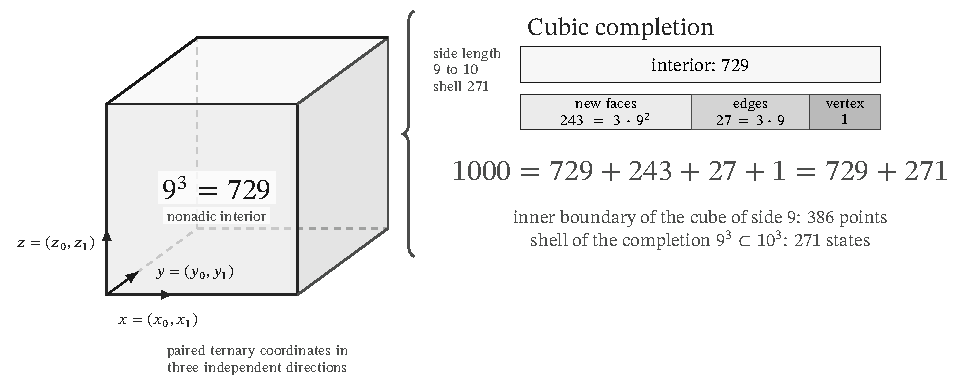
\includegraphics[width=\linewidth]{figures/cubo_emrh.pdf}
\caption{Cubic representation of the expansion from nine to ten classes per coordinate. Strata \(S_1,S_2,S_3\) locate the added incidences on faces, edges, and the apex; their cardinalities form the \(271\)-element shell. The \(386\)-element boundary belongs to the initial cube. This geometric perspective complements the partition in Figure~\ref{fig:revision-emrh}; graphical spacing is schematic.}
\label{fig:completacion-cubo-recuperado}
\end{figure}


\subsubsection{Preservation of unity and dimensional compatibility}

Normalization is not limited to dividing an isolated identity. In dimension
\(d\), the product \(\widehat E^d\) carries the uniform measure
\(\mu_d(\{x\})=10^{-d}\). The coordinate projection
\(p_d:\widehat E^{d+1}\to\widehat E^d\) deletes the final coordinate.

\begin{proposition}[Projective compatibility of the normalized measures]
For every \(d\geq1\),
\[
 (p_d)_*\mu_{d+1}=\mu_d,
 \qquad \mu_d(\widehat E^d)=1.
\]
The mass of the stratum with \(r\) additional coordinates is
\(\binom dr9^{d-r}/10^d\), and the sum of the masses of all strata
is one.
\end{proposition}
\begin{proof}
Every point of \(\widehat E^d\) has ten preimages. Their total mass is
\(10\,10^{-(d+1)}=10^{-d}\). Equality for any subset
is obtained by summing over its points. The stratified formula follows
from the same count as \eqref{eq:revision-estratos}; the binomial
\((9+1)^d\) gives the total normalization.
\end{proof}

In dimension three, removing the apex leaves mass \(999/1000\), and
restoring it adds \(1/1000\). Renormalizing before restoration
would define a different measure: the distinction is operationally relevant.
In particular, preservation of probability mass, preservation of
transport records, and thermodynamic dissipation are assertions concerning
different objects. The proposition proves the first and provides the
compatible support for studying the second; the third requires a
specified dynamical and energetic realization.

The internal geometric boundary likewise remains distinct.
On the Cartesian representative \(\{1,\ldots,9\}^3\), removing
\(\{2,\ldots,8\}^3\) leaves \(386\) points. This boundary belongs to the
initial cube, whereas \(\widehat C\setminus C\) belongs to its
enlargement. The cubic completion, the base-one-thousand positional expansion,
and the exceptional-incidence reading share support data;
their respective maps determine which information from those data is used by
each representation.
